%%%%%%%%%%%%%%%%%%%%%%%%%%%%%%%%%%%%%%%%%
% University Assignment Title Page 
% LaTeX Template
% Version 1.0 (27/12/12)
%
% This template has been downloaded from:
% http://www.LaTeXTemplates.com
%
% Original author:
% WikiBooks (http://en.wikibooks.org/wiki/LaTeX/Title_Creation)
%
% License:
% CC BY-NC-SA 3.0 (http://creativecommons.org/licenses/by-nc-sa/3.0/)
% 
% Instructions for using this template:
% This title page is capable of being compiled as is. This is not useful for 
% including it in another document. To do this, you have two options: 
%
% 1) Copy/paste everything between \begin{document} and \end{document} 
% starting at \begin{titlepage} and paste this into another LaTeX file where you 
% want your title page.
% OR
% 2) Remove everything outside the \begin{titlepage} and \end{titlepage} and 
% move this file to the same directory as the LaTeX file you wish to add it to. 
% Then add \input{./title_page_1.tex} to your LaTeX file where you want your
% title page.
%
%%%%%%%%%%%%%%%%%%%%%%%%%%%%%%%%%%%%%%%%%

%----------------------------------------------------------------------------------------
%	PACKAGES AND OTHER DOCUMENT CONFIGURATIONS
%----------------------------------------------------------------------------------------

\documentclass[12pt]{article}
\usepackage{graphicx}
\begin{document}

\begin{titlepage}

\newcommand{\HRule}{\rule{\linewidth}{0.5mm}} % Defines a new command for the horizontal lines, change thickness here


 
%----------------------------------------------------------------------------------------

\center % Center everything on the page
 
%----------------------------------------------------------------------------------------
%	HEADING SECTIONS
%----------------------------------------------------------------------------------------


%----------------------------------------------------------------------------------------
%	LOGO SECTION
%----------------------------------------------------------------------------------------


\includegraphics{logo_epfl-eps-converted-to}\\[1cm] % Include a department/university logo - this will require the graphicx package

%\textsc{\LARGE \'Ecole Polytechnique F\'ed\'erale de Lausanne}\\[1.5cm] % Name of your university/college
\textsc{\Large Biological Modeling of Neural Networks}\\[0.5cm] % Major heading such as course name

%----------------------------------------------------------------------------------------
%	TITLE SECTION
%----------------------------------------------------------------------------------------

\HRule \\[0.4cm]
{ \huge \bfseries Hopfield Model}\\[0.4cm] % Title of your document

\textsc{\large Storage of Sequences of patterns in asymetric hopfield networks with delayed synapses}\\[0.5cm] % Minor heading such as course title

\HRule \\[1.5cm]

%----------------------------------------------------------------------------------------
%	AUTHOR SECTION
%----------------------------------------------------------------------------------------

\begin{flushright}
\large Miryam \textsc{Chaabouni}

\large Joseph \textsc{Lemaitre}\\ % Your name

\end{flushright}


% If you don't want a supervisor, uncomment the two lines below and remove the section above
%\Large \emph{Author:}\\
%John \textsc{Smith}\\[3cm] % Your name

%----------------------------------------------------------------------------------------
%	DATE SECTION
%----------------------------------------------------------------------------------------

%{\large \today}\\[3cm] % Date, change the \today to a set date if you want to be precise

\vfill % Fill the rest of the page with whitespace

\end{titlepage}

\section{Exercise 1 : Standard Hopfield Network }
\subsection{Exercise 1.1 : Implementation}
We created a class hopfieldNetwork which has the following attributes : 
\begin{itemize}
\item N : number of neurons 
\item pattern : array of $P\times N$ states, where P is the number of patterns 
\item weight : array of $N\times N$ that represents the matrix of interaction between neurons
\item x : state of the network at each time step, e.g.,  $x = \{1, -1, -1, \dots\}$
\end{itemize}
and the following functions : 
\begin{description}
\item [\_\_init\_\_] creates an instance of the class hofieldNetwork with the number of neurons N 
\item [makePattern] creates a numpy array of N$\times$P of ones, then randomly flips a given ratio of neurons in each pattern using the function numpy.random.choice. 
\item [makeWeight] calculates the interaction weights using simple for loops according to the formula : $w_{ij} = \frac{1}{N}\sum_{m=1}^P \xi_i^{\mu} \xi_j^{\mu}$
\item[dynamic] updates the state of neuron i according to the formula : $S_i = \textrm{sign}\big(\sum_{j=1}^N w_{ij}S_j\big)$ using the weight matrix and the current state of the network

\end{description}

After creating an instance of the class hopfieldNework and creating the desired number of patterns, we run the simulation using the run function which does the following steps : 
\begin{enumerate}
\item initialize the network by copying one of the patterns $\xi^{\mu}$ then flipping the state of randomly chosen neurons 
\item Select a random neuron and update its state using the dynamic function, and do this for all the neurons of the network
\item repeat until convergence
\end{enumerate}
For the convergence criterion, we store the value of the network x at each step, and after each iteration we compare the old value of x to the new one by a simple subtraction. If the difference is negligible, we stop. In addition, we set a time limit tmax = 100 steps, so that we exit even if the model doesn't converge. \\
The runAndPlot function performs the same steps as run, but plot at the same time the network and illustrates the convergence in a overlap w.r.t. time curve. \\
At each time step, we store the value of the overlap and the normalized pixel distance which will be useful later. \\
 
\subsection{Exercise 1.2 : Pattern retrieval }
At this step we add two functions : 
\begin{description}
\item [overlap] calculates the overlap between the pattern $\xi^{\mu}$ and the current state of the network according to the formula : $m^{\mu} = \frac{1}{N}\sum_{i=1}^N \xi_i^{\mu}S_i(t)$
\item[pixeldistance] calculates the percentage of neurons in the network that differ from the pattern $\xi^{\mu}$ using the formula : $(1-m^{\mu}) \times 100$, where $m^{\mu}$ is the overlap returned by the aforementioned function. 
\end{description}

To get the retrieval error as a function of the ratio $c$ of the flipped bits at the initialization of the network, we define the function patternRetrieval. \\
We fix N=200 and P = 5. We take 50 values of c in the interval [0.01, 0.51]. For each value of c, we get run the simulation 50 times, and get the pixel distance at the end of each simulation. We show the average of the retrieval error in figure \ref{reterr}. The error bar represents the standard error of the mean, and is given by SciPy function stats.sem. \\
As we could expect it, the error is negligible ($<1\%$) if we flip a reasonable ratio of the neurons at the initialization step. According to the figure, this threshold value is $c = 0.35$. As the number of flipped neurons increases, the error grows exponentially. For $c=0.5$, meaning that we start with a network where half of the neurons are different from the retrieved pattern, the error reaches 100$\%$. \\
(What happens when m=-1???)\\
We conclude that the Hopfield model works well only if the initial state of the Network is close to the target pattern.
\begin{center}
    \begin{figure}\label{reterr}
    \caption{Mean retrieval error as a function of the flip ration $c\in[0.01, 0.51]$.  }
    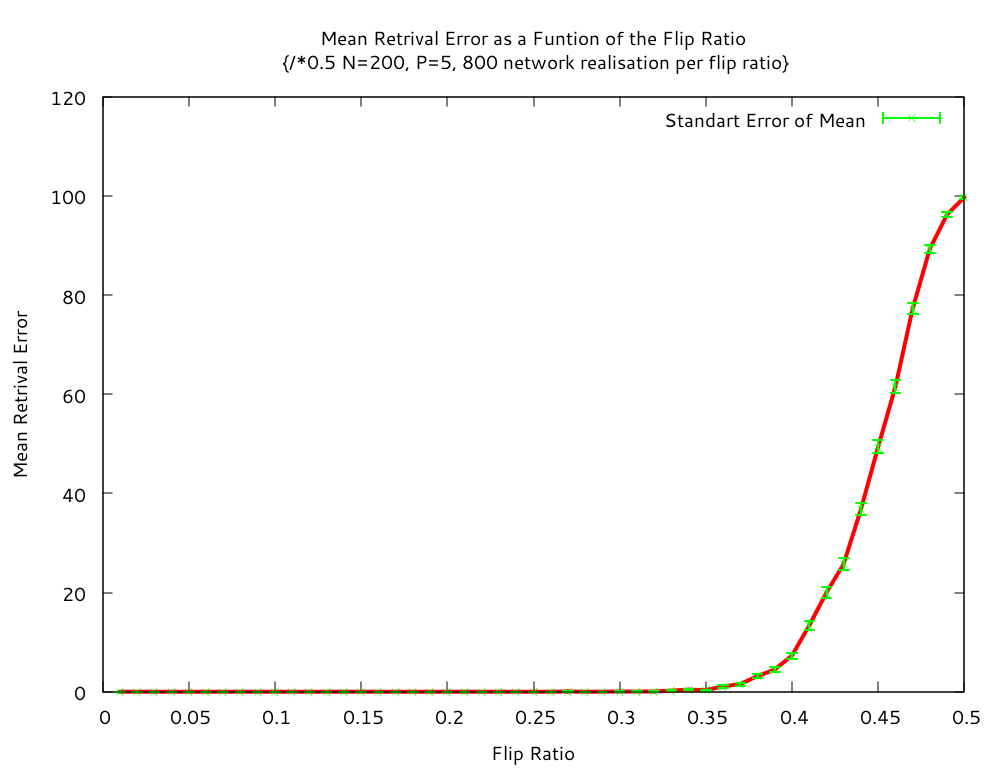
\includegraphics[scale=0.7]{img/ex11.png}
    \end{figure}
\end{center}

\subsection{Exercise 1.3 : Capacity estimation}
The number of patterns that can be stored and retrieved correctly by a neurons network depends on the number of neurons. In Hofield model, the storage capacity of a network is defined by :
\begin{equation}\nonumber
C_{stor} =\frac{ P^{max}}{N}
\end{equation} 
where $P^{max}$ is the maximum number of patterns that the network can retrieve correctly. \\
To study this capacity, we define the function maxLoad. To obtain the capacity of the Hopfield Network, we create a network of N neurons and a growing number of patterns $P \leq 51$.  We fix $c=0.1$. For each $P$ we try to retrieve a random pattern 10 times and we get the mean error. When the mean error reaches $2\%$ we stop and save the number of patterns created $P_{max}$. To speed up the simulation, we start from P=???. Finally, we calculate the average value of $P_{max}$ for a given $N$, and we calculate the maximal load $\alpha_{max} = P_{max}/N$. We will do this for several values of N. The results are shown in table \ref{capa}.  
\begin{table}[h]\label{capa}
\begin{center}
\begin{math}
    \begin{array}{|l|c|c|c|}
    \hline
    N & 100 & 250 & 500 \\ \hline
    P_{max} & 17 & 39 &  \\ \hline
    \alpha_{max} & 0.17 & 0.156 & - \\ \hline
    \alpha_{th} & - & - & - \\ \hline
    \end{array}
\end{math}
\end{center}
\caption{Capacity storage of a network of N neurons }
\end{table}
The error on the value of $\alpha_{max}$ is calculated by ... \\
As we could expect, we observe that the capacity of the network increases with the number of neurons. Moreover, we see that the maximal load that we obtain corresponds extremely well to the theoretical value.\\
Note that we only retrieve one pattern at a time. If we want to retrieve a sequence of patterns, the literature says that $C_{stor}$ should not exceed 0.138\cite{prof}, otherwise, the error will propagate at each pattern of the sequence. From our table, we see that this threshold is exceeded for N=250 and N=500. Therefore, we should to modify the model if we want to retrieve a sequence of patterns. 
\section{Exercise 2}
\subsection{Exercise 2.2}
We used the heaviside filter function. We had a bit
of freedom to define {\it sequencial behaviour}. We decreased lambda to get the minimum value
for which all pattern are visited. We found :
\begin{center}
$\lambda_{min} \approx 0.9$
\end{center}
For values below this one, the network get stuck in a particular pattern. Due to the random generation
of some variables, the value of $\lambda_{min}$ is approximative.


For the calculus of $\lambda_{max}$, we saw that for high lambda the network jump over some frame, not
getting an overlap of one. Therefore we defined the sequencial behaviour as all state are visited with a overlap of 1, 
one after each other.
We found :
\begin{center}
$\lambda_{max} = 3.6$
\end{center}
\subsection{Exercice 2.3}

\subsection{Exercice 2.4 : Sequence Storage Capacity}

By varying $P$ with $N$ fixed, we saw that increasing the number of pattern stored lead the network
to never acheive an overlap of $1$, or only for a few pattern (with $N = 500$ and $P = 40$ for example, only pattern, the $4$,
was retrieved correctly). If we print the overlap we see that for a high $P$, the mean overlap is considerably lower (only 22 out of 400
iteration sees their overlap over $0.7$ for $N = 500$ and $P = 50$, this number was 375 with the same setup, for $P = 10$). So transition
from fully recovered patterns are our control behaviour to test the number of pattern we can store. 

We fixed all the parameter of our network, except the number of pattern $P$ and the size of the
network $N$. We then moved $P$ until one of the pattern stored was missed during an interation (this is our criterion
but several can be chosen, like a threshold with the transition time between two pattern that get very long
with $P$). The results are displayed on Table~\ref{capaseq}. Again due to the randomness of the process
we show here statistical average, but on too few sample to be sure. 

\begin{table}[h]\label{capaseq}
\begin{center}
\begin{math}
    \begin{array}{|l|c|c|c|}
    \hline
    N & 250 & 500 & 1000 \\ \hline
    P_{max} & 15 & 33 & 52 \\ \hline
    \alpha_{max}& 0.06 & 0.066 & 0.052\\ \hline
    \end{array}
\end{math}
\end{center}
\caption{Sequence storage capacity  of a network of N neurons}
\end{table}
 We can compare those results to 


\begin{thebibliography}{}
\bibitem{prof} W. Gerstner, W. Kistler, R. Naud, L. Paninski, \textit{Neuronal Dynamics : from single neurons to networks and models of cognition}, Cambridge University Press, 2014.
\end{thebibliography}
\end{document}